\chapter{Laporan}
\section{Teori}
\subsection{Sejarah Python}
Guido van Rossum merupakan pencipta Bahasa python pertama kali di Centrum Wiskunde dan Informatica (CWI) pada awal tahun 1990-an di Belanda. Python merupakan Bahasa pemrogaman tigkat tinggi.Bahasa Python terinsipirasi dari Bahasa pemrogaman ABC. Python bersifat open source sehingga ribuan orang banyak yang berkontribusi dalam mengembangkannya. Tahun 1995, Guido melanjutkan untuk mengembangkan python di Corporation for National Research Initiaive (CNRI) di Virgina Amerika dan dia berhasil merilis beberapa versi dari python.Pada mei 2000, Guido dan tim Python pindah BeOpen.com dan membentuk tim BeOpen PythonLabs dan Pada bulan oktober pda tahun yg sama,tim python pindah ke Digital Creation  sehingga pada tahun 2001 dibentiuklah organisasi python yaitu Python Software Foundation (PSF). PSF dibentuk khusus untuk semua hal yg berkaitan dengan intelektual Python. Dan semua python yang dirilis bersifat open source. 
\subsection{Perbedaan Python 2 dan Python 3}
Python 2
	\begin{enumerate}
		\item untuk membuka Bahasa pemrogaman python 2 kita hanya menggunakan perintah python saja
		\item dan python 2 bagus untuk belajar bagi pemula.
	\end{enumerate}
	\hfill \break
Python 3
	\begin{enumerate}
		\item untuk membuka python 3 dengan menggunakan perintah python3. 
		\item python 3 digunakan bagi yang sudah mahir
	\end{enumerate}
\subsection{Implementasi dan penggunaan Python di perusahaan dunia}
Python banyak digunakan di perusahan di dunia karena python memiliiki sintaks Bahasa pemrogaman yang sederhana dan mudah dimengerti. Sudah banyak perusahaan yang menggunakan Bahasa python untuk pembuatan programnya mulai dari Perusahan Google, Yahoo!,Instagram,Pinterest,Youtube, hingga Reddit. Python juga sudah dimanfaatkan oleh NASA. Untuk penggunaan Python dalam Analisis Data bisa dilihat dalam platform seperti Spotify dan Netflix. Penerapan dalam kedua platform digital ini, dapat terlihat utamanya yaitu bagaimana Spotify merekomendasikan lagu dan Netflix merekomendasikan film kepada para pelanggannya.
\subsection{Instalasi}
\subsubsection{Instalasi python}
Berikut merupakan tahapan-tahapan untuk menginstall python:
	\begin{figure}[H]
		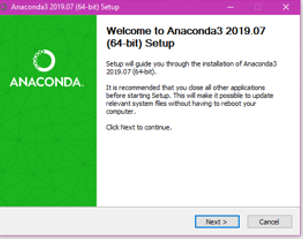
\includegraphics[width=4cm]{figures/1184065/4.PNG}
		\centering
		\caption{Buka software Anaconda3 yang telah di download terlebih dahulu}
	\end{figure}
	\begin{figure}[H]
		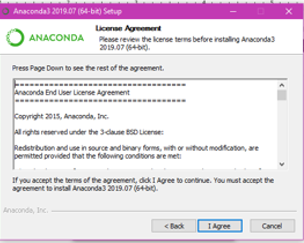
\includegraphics[width=4cm]{figures/1184065/5.PNG}
		\centering
		\caption{klik i agree untuk memberikan license agreement}
	\end{figure}
	\begin{figure}[H]
		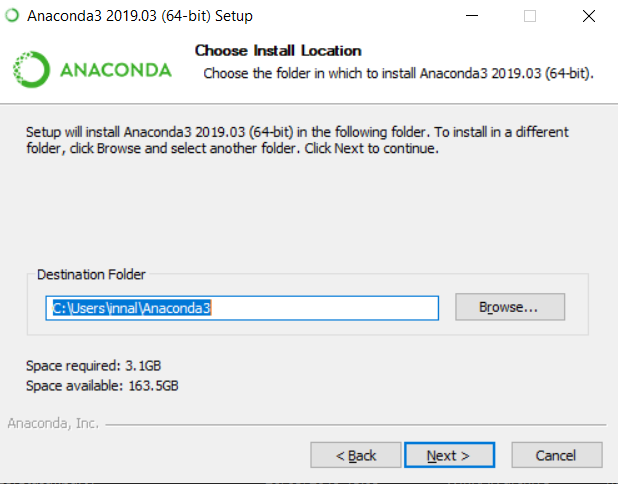
\includegraphics[width=4cm]{figures/1184065/6.PNG}
		\centering
		\caption{Pilih salah satu untuk menginstall, pilih just me atau all users}
	\end{figure}
	\begin{figure}[H]
		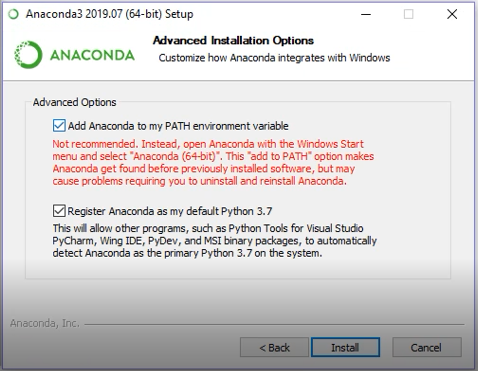
\includegraphics[width=4cm]{figures/1184065/7.PNG}
		\centering
		\caption{pilih lokasi untuk menginstall software }
	\end{figure}
	\begin{figure}[H]
		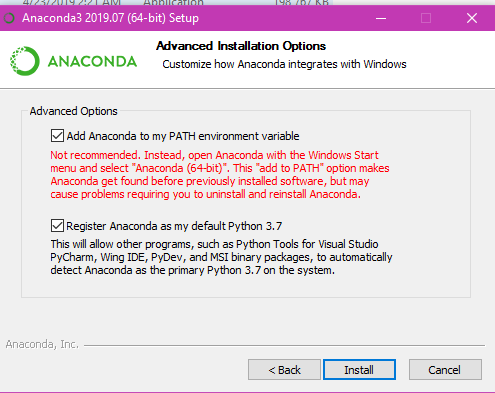
\includegraphics[width=4cm]{figures/1184065/addNew.PNG}
		\centering
		\caption{Beri tanda centang pada dua kolom yang telah disediakan. }
	\end{figure}
	\begin{figure}[H]
		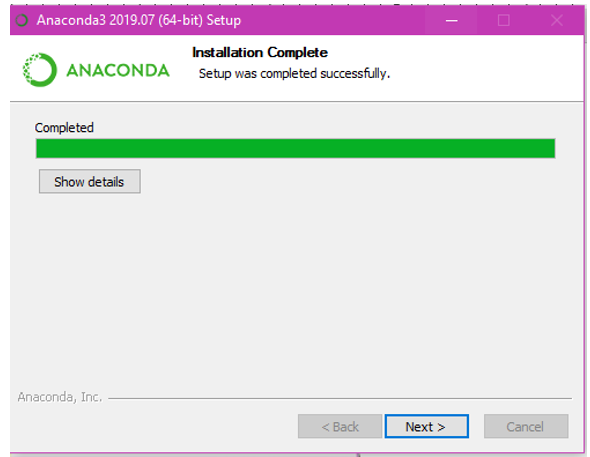
\includegraphics[width=4cm]{figures/1184065/9.PNG}
		\centering
		\caption{Instalasi anaconda sedang dalam proses berjalan}
	\end{figure}
	\begin{figure}[H]
		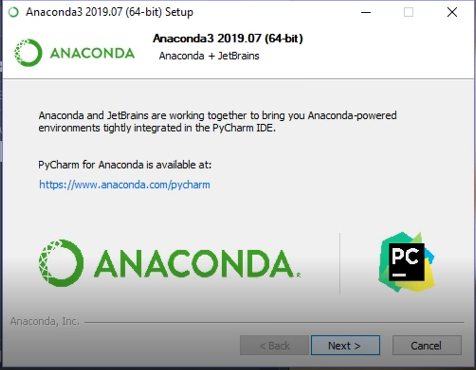
\includegraphics[width=4cm]{figures/1184065/10.PNG}
		\centering
		\caption{Klik next untuk melanjutkan proses instalasi}
	\end{figure}
	\begin{figure}[H]
		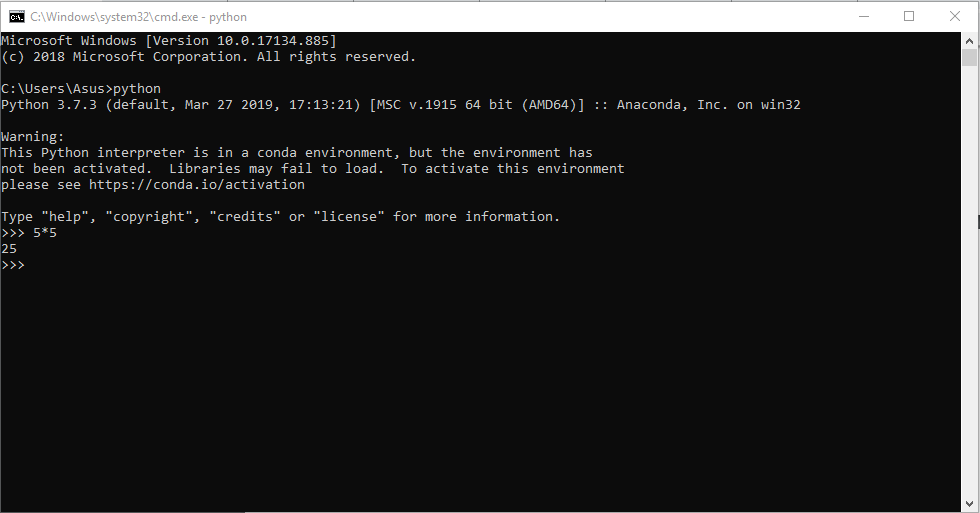
\includegraphics[width=4cm]{figures/1184065/11.PNG}
		\centering
		\caption{Anaconda yang di dalamnya sudah terdapat python berhasil diinstal, dan siap digunakan}
	\end{figure}
\subsubsection{Instalasi pip}
Berikut merupakan langkah-langkah untuk menginstall pip:
	\begin{figure}[H]
		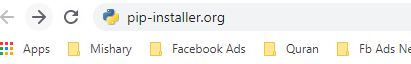
\includegraphics[width=4cm]{figures/1184065/downloadPIP.PNG}
		\centering
		\caption{Pertama-tama kalian harus mengunjungi website resmi PIP yaitu pip-installer.org}
	\end{figure}
	\begin{figure}[H]
		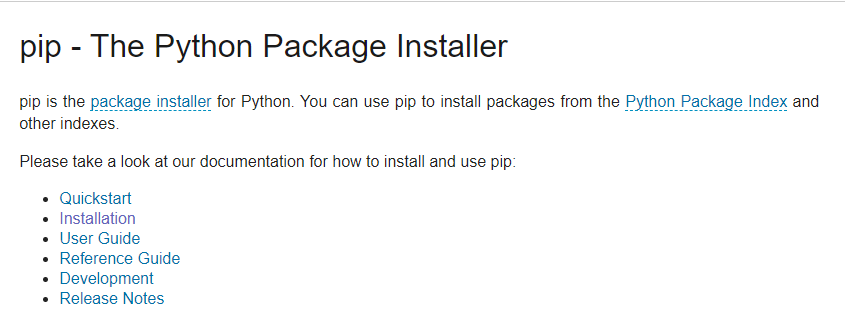
\includegraphics[width=4cm]{figures/1184065/PilihInstaller.PNG}
		\centering
		\caption{Klik Installatation pada package}
	\end{figure}
	\begin{figure}[H]
		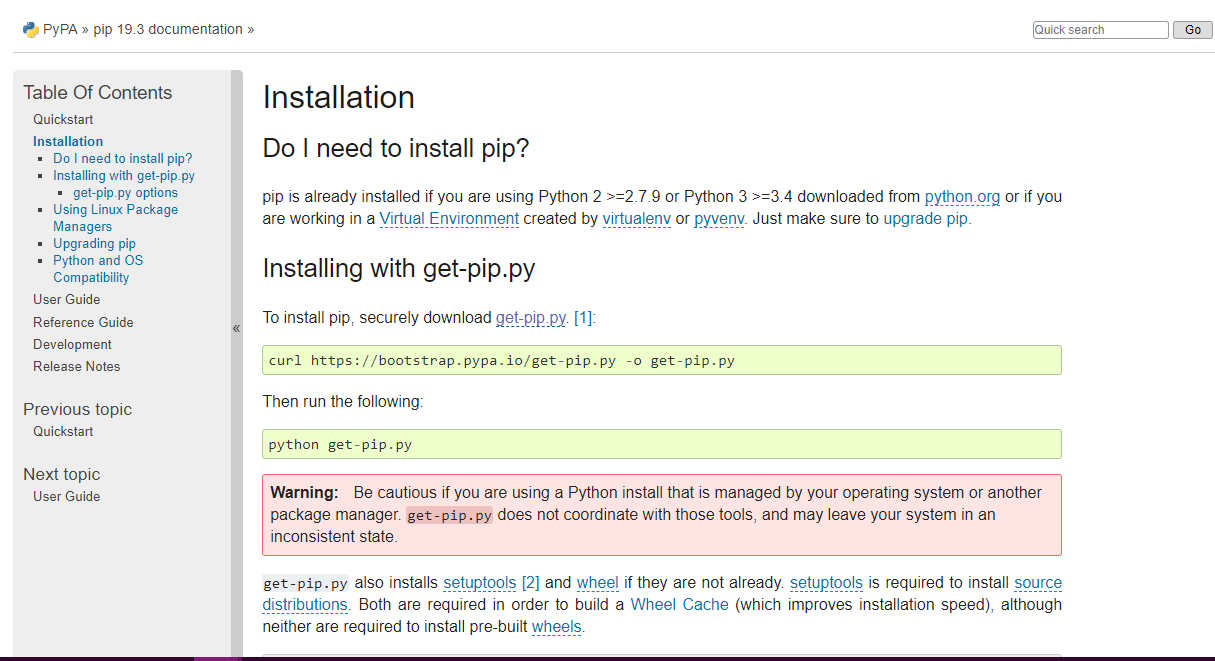
\includegraphics[width=4cm]{figures/1184065/KlikGetPip.PNG}
		\centering
		\caption{anda akan diarahkan untuk mendownload pip klik get-pip.py lalu klik kanan dan klik save link as dan simpan download-an PIP sesuai lokasi file yg anda inginkan}
	\end{figure}
	\begin{figure}[H]
		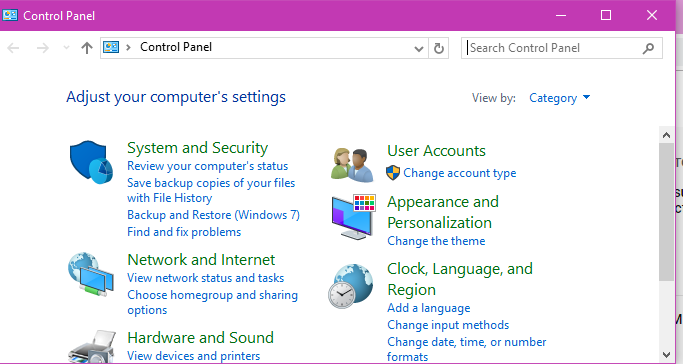
\includegraphics[width=4cm]{figures/1184065/SystemPIP.PNG}
		\centering
		\caption{Kemudian setelah selesai download PIP anda masuk ke dalam control panel dan klik system dan security lalu klik system }
		\end{figure}
		\begin{figure}[H]
		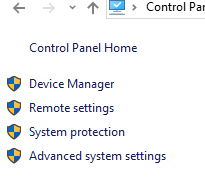
\includegraphics[width=4cm]{figures/1184065/PIPAdvanced.PNG}
		\centering
		\caption{setelah masuk ke system anda klik Advanced system settings}
	\end{figure}
	\begin{figure}[H]
		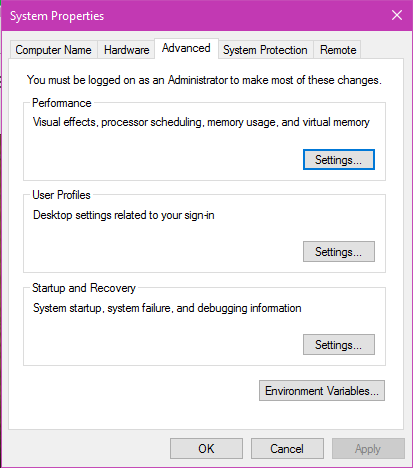
\includegraphics[width=4cm]{figures/1184065/EnvironmentVar.PNG}
		\centering
		\caption{lalu akan muncul sebuah tampilan dan klik Environment Variables }
	\end{figure}
	\begin{figure}[H]
		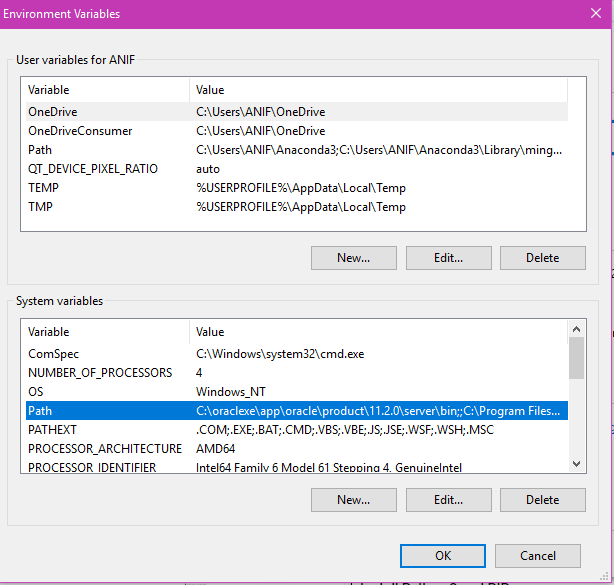
\includegraphics[width=4cm]{figures/1184065/EnvironmentPath.PNG}
		\centering
		\caption{lalu akan muncul sebuah tampilan System Variables dan klik path lalu klik edit}
	\end{figure}
	\begin{figure}[H]
		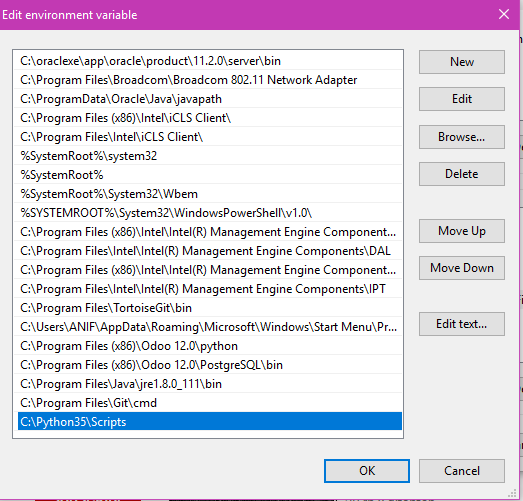
\includegraphics[width=4cm]{figures/1184065/TambahPython35.PNG}
		\centering
		\caption{Setelah itu klik new lalu tambahkan lokasi Python seperti pada gambar}
	\end{figure}
	\begin{figure}[H]
		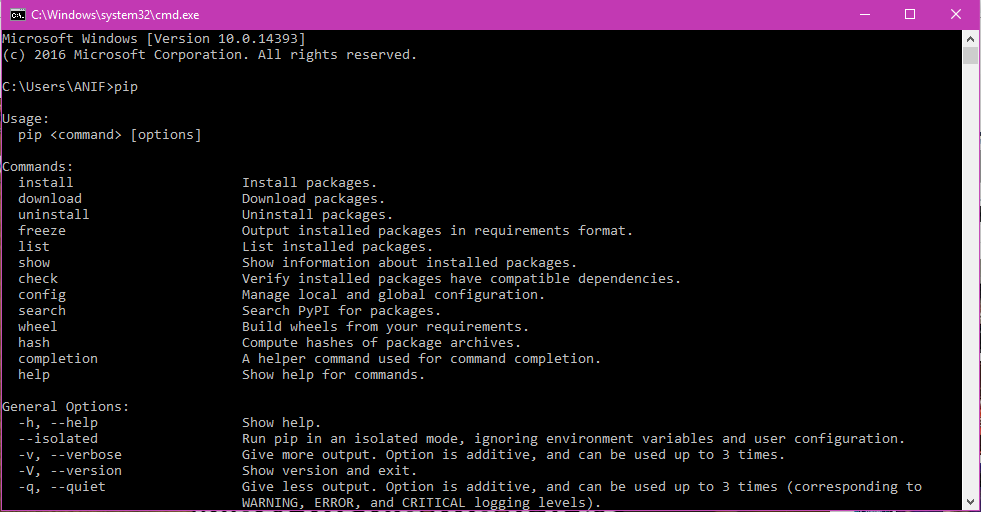
\includegraphics[width=4cm]{figures/1184065/HasilPIP1.PNG}
		\centering
		\caption{Instalasi siap digunakan, lalu untuk mengecek apakah aplikasi sudah terinstal atau belum bisa menggunaknan perintah pip pada cmd}
	\end{figure}
	\begin{figure}[H]
		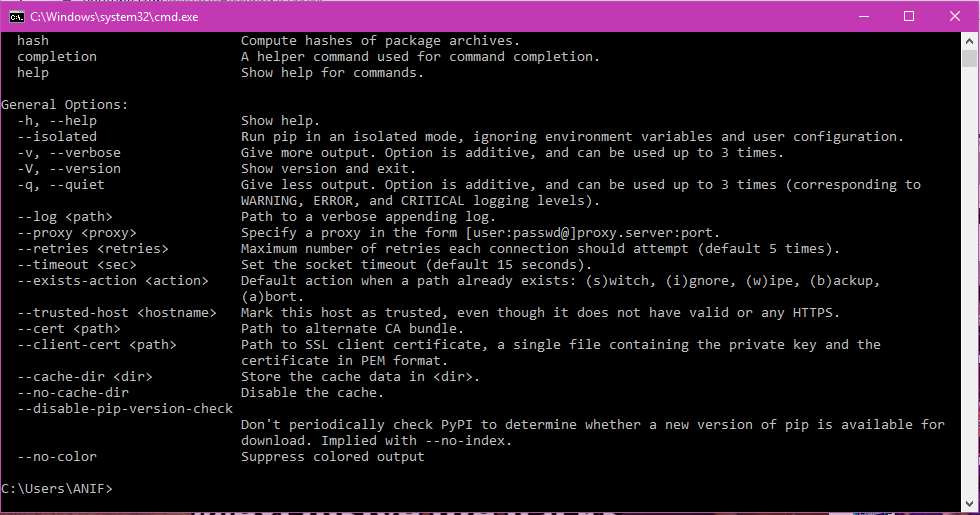
\includegraphics[width=4cm]{figures/1184065/HasilPIP2.PNG}
		\centering
		\caption{Instalasi siap digunakan, lalu untuk mengecek apakah aplikasi sudah terinstal atau belum bisa menggunaknan perintah pip pada cmd}
	\end{figure}      
\subsubsection{Cara setting environment}
	\begin{figure}[H]
		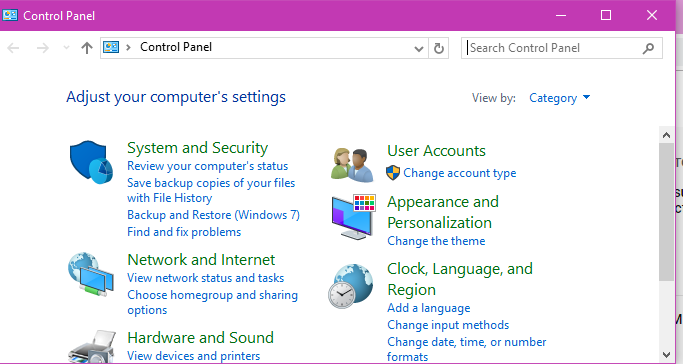
\includegraphics[width=4cm]{figures/1184065/SystemPIP.PNG}
		\centering
		\caption{untuk setting environment pertama kita buka control panel terlebih dahulu lalu klik system and security lalu masuk ke system}
	\end{figure}
	\begin{figure}[H]
		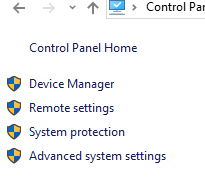
\includegraphics[width=4cm]{figures/1184065/PIPAdvanced}
		\centering
		\caption{Setelah masuk ke dalam system maka lanjut klik Advanced System settings}
	\end{figure}
	\begin{figure}[H]
		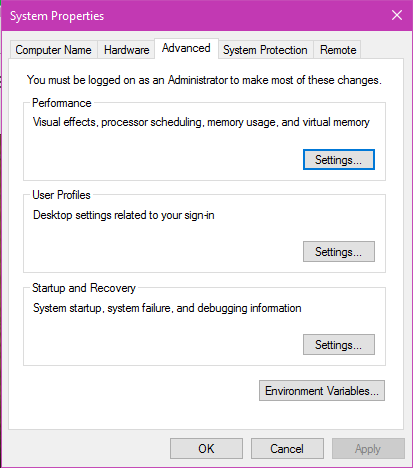
\includegraphics[width=4cm]{figures/1184065/EnvironmentVar.PNG}
		\centering
		\caption{Setelah masuk ke Advanced System settings akan muncul tampilan System properties lalu klik environment}
	\end{figure}
	\begin{figure}[H]
		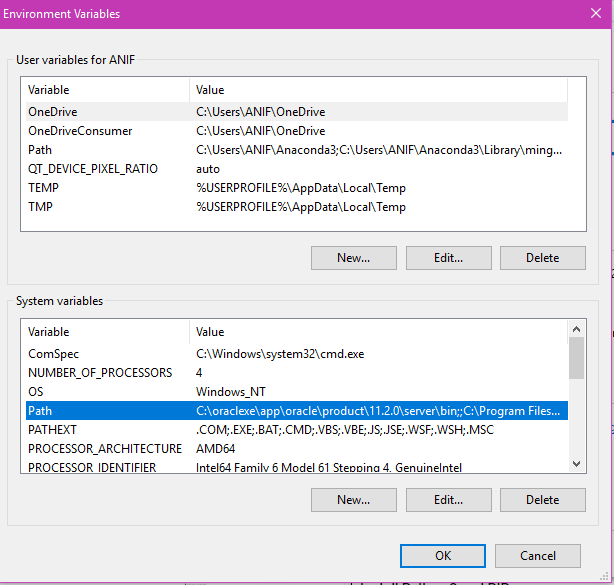
\includegraphics[width=4cm]{figures/1184065/EnvironmentPIP.PNG}
		\centering
		\caption{Setelah masuk ke Advanced System settings akan muncul tampilan system variables dan klik ok}
	\end{figure}
\subsubsection{Mencoba enterpreter/cli melalui terminal atau cmd windows}
Berikut merupakan langkah-langkah untuk mencoba enterpreter melalui terminal atau cmd windows:
\begin{figure}[H]
		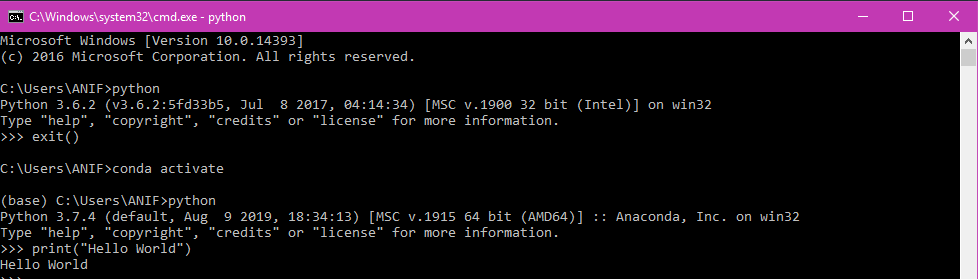
\includegraphics[width=4cm]{figures/1184065/EnterpreterNew.PNG}
		\centering
		\caption{gambar diatas merupakan kodingan enterpreter malalui cmd windows, pertama kalian harus tulis perintah Python terlebih dahulu untuk mengetahui versi dari python itu sendiri, kemudian tuliskan exit() untuk keluar karena conda environmentnya bekum aktif lalu ketik ulang perintah python di cmd dan aktifkan conda environmenya dengan perintah conda activate kemudian tuliskan perintah untuk mencetak hasil dengan perintah "print" }
	\end{figure}
\subsubsection{Menjalankan dan mengupdate anaconda dan spyder}
Berikut merupakan langkah-langkah untuk menjalankan dan mengupdate anaconda dan spyder:
\begin{figure}[H]
		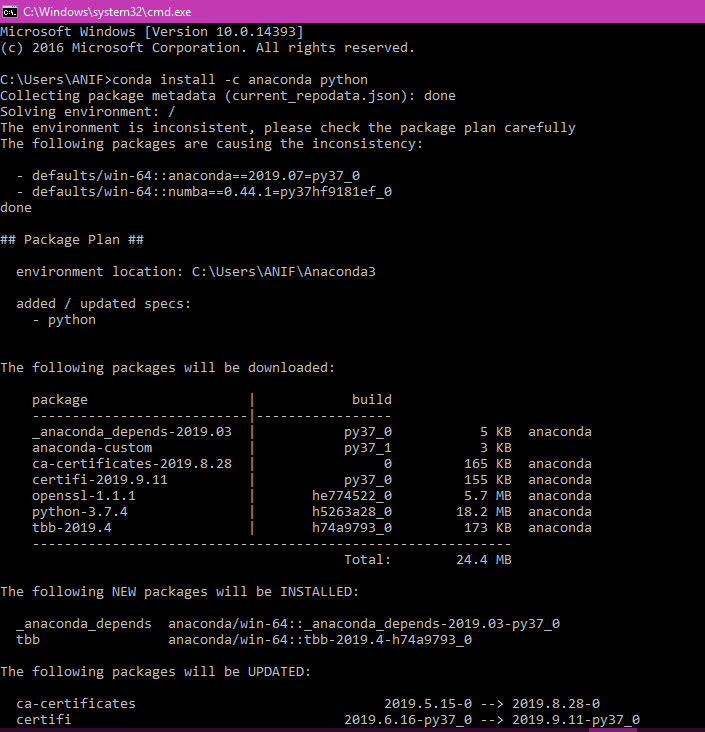
\includegraphics[width=4cm]{figures/1184065/UpdateAnacondaNew1.PNG}
		\centering
		\caption{Untuk pertama-tama kalian harus menuliskan script conda install -c anaconda python pada cmd lalu enter}
	\end{figure}
	\begin{figure}[H]
		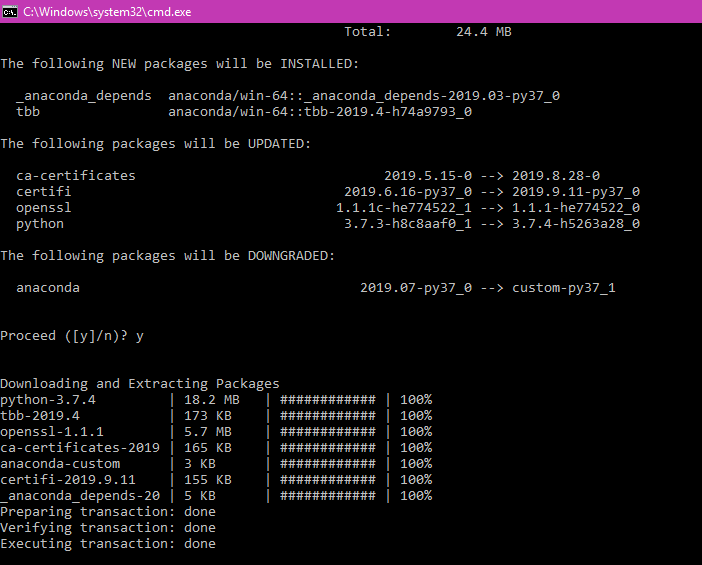
\includegraphics[width=4cm]{figures/1184065/UpdateAnacondaNew2.PNG}
		\centering
		\caption{Setelah selesai menjalankan script tersebut, kalian akan diberikan 2 perintah pilihan yaitu perintah y/n dan kalian harus menuliskan perintah y tunggu hingga semua proses done dan anaconda berhasil terupdate}
	\end{figure}
	\begin{figure}[H]
		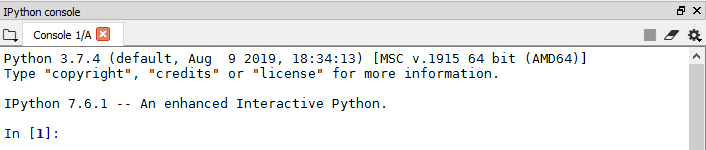
\includegraphics[width=4cm]{figures/1184065/UpdateSpyder.PNG}
		\centering
		\caption{Setelah selesai mengupdate anaconda pada cmd tersebut, anda dapat melihat versi spyder anda berubah di dalam spyder. yang tadinya spyder versi 3.7.3 menjadi 3.7.4}
	\end{figure}
	
\subsubsection{Cara menjalankan Script Hello World di spyder}
\begin{figure}[H]
		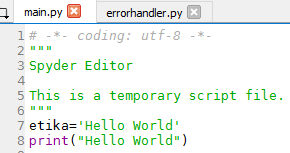
\includegraphics[width=4cm]{figures/1184065/PerintahHelloWorld.PNG}
		\centering
		\caption{gambar diatas merupakan perintah atau koding untuk menampilkan hasil tulisan Hello World }
	\end{figure}
\begin{figure}[H]
		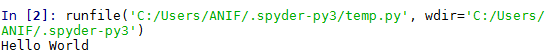
\includegraphics[width=4cm]{figures/1184065/Hasil_Hello_World.PNG}
		\centering
		\caption{gambar diatas merupakan semacam pemberitahuan berhasil dari perintah tulisan Hello World }
	\end{figure}
\subsubsection{Cara menjalankan Script otomatis login aplikasi akademik dengan library selenium dan inputan user}
Berikut merupakan langkah-langkah untuk menjalankan login otomatis pada aplikasi akademik library selenium:
\begin{figure}[H]
		
\includegraphics[width=4cm]{figures/1184065/Gecko.PNG}
		\centering
		\caption{Sebelum mendownload selenium pada cmd kalian harus mendownload geckodriver.exe terlebih dahulu. Setelah itu save aplikasi geckodriver tersebut dalam windows C }
	\end{figure}
\begin{figure}[H]
		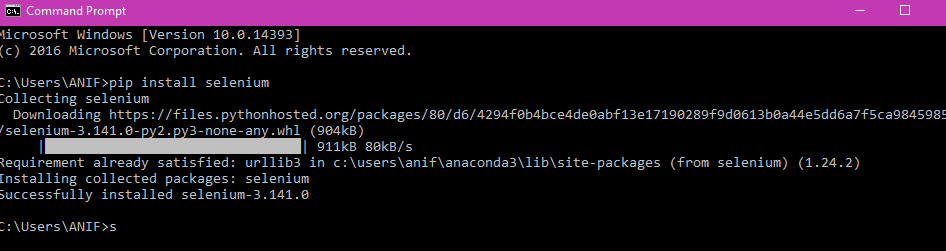
\includegraphics[width=4cm]{figures/1184065/Selenium1.PNG}
		\centering
		\caption{gambar diatas merupakan langkah utama untuk bisa menjalankan login otomatis pada aplikasi akademik library selenium kalian harus mendownload selenium terlebih dahulu dengan cara tulis script pip install selenium pada cmd kemudian enter}
	\end{figure}
\begin{figure}[H]
		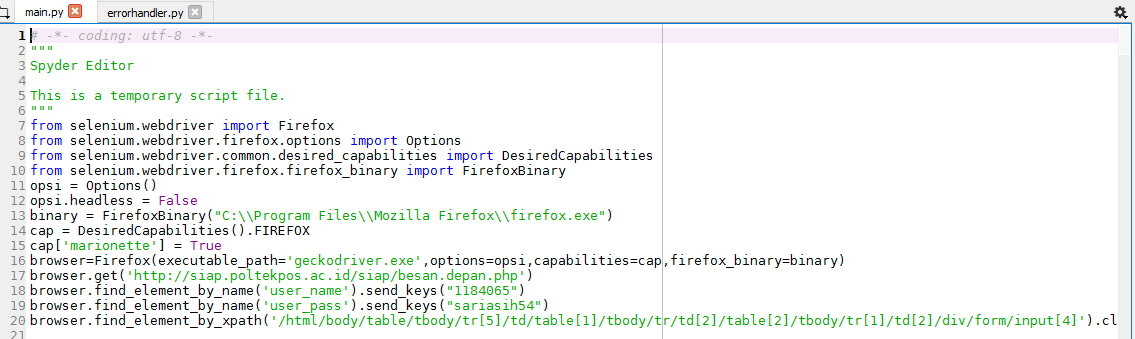
\includegraphics[width=4cm]{figures/1184065/KodingPenggunaOtomatis.PNG}
		\centering
		\caption{untuk menjalankan script login otomatis pada aplikasi akademik library selenium kalian dapat menggunakan spyder }
	\end{figure}
	\begin{figure}[H]
		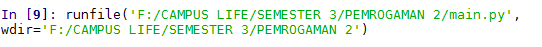
\includegraphics[width=4cm]{figures/1184065/KeteranganLoginOtomatis.PNG}
		\centering
		\caption{gambar diatas merupakan semacam pemberitahuan jika script login otomatis aplikasi akademik library selenium berhasil dijalankan}
	\end{figure}
	\begin{figure}[H]
		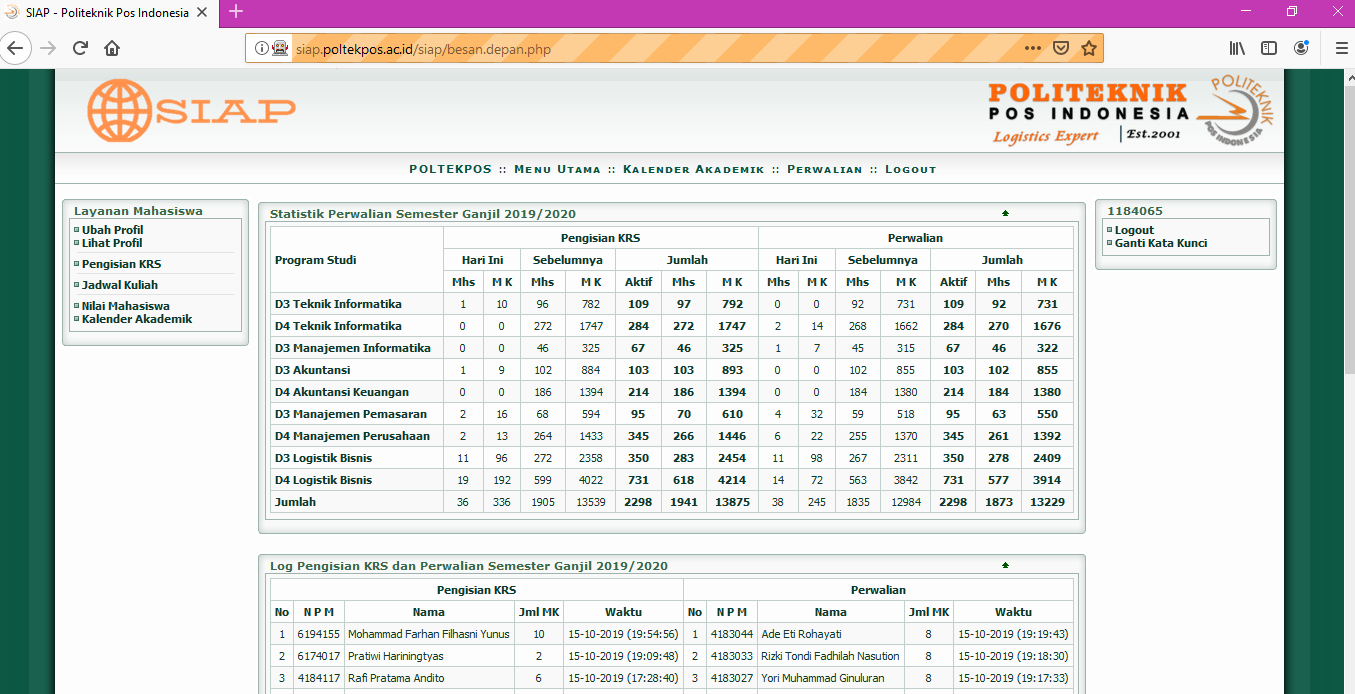
\includegraphics[width=4cm]{figures/1184065/HasilLoginOtomatis.PNG}
		\centering
		\caption{gambar diatas merupakan hasil dari login otomatis yg berhasil ke dalam aplikasi SIAP }
	\end{figure}
\subsubsection{Cara menjalankan pemakaian variable explorer di spyder}
 Berikut merupakan langkah-langkah untuk menjalankan variable explorer:
\begin{figure}[H]
		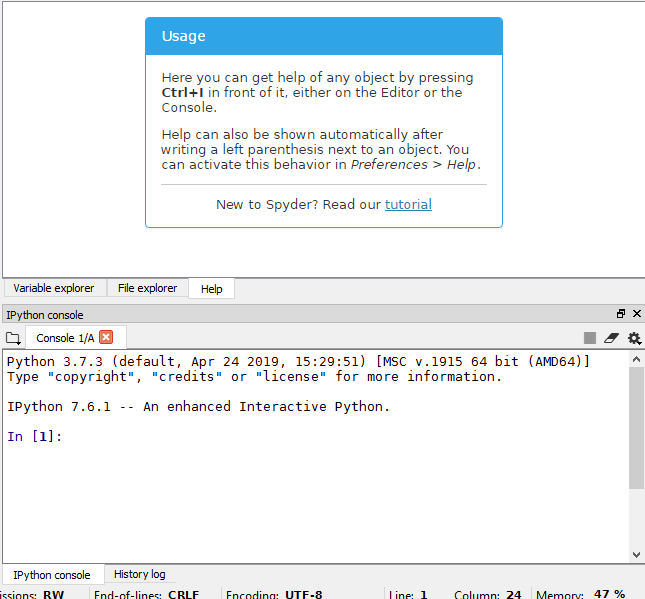
\includegraphics[width=4cm]{figures/1184065/Variable_explorer.PNG}
		\centering
		\caption{gambar diatas merupakan langkah pertama untuk membuka variable explorer dalam spyder. klik bagian bawah kiri yang terdapat tulisan Variable explorer }
	\end{figure}
	\begin{figure}[H]
		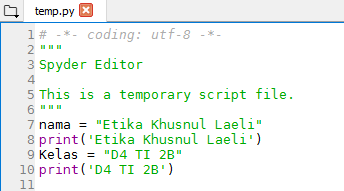
\includegraphics[width=4cm]{figures/1184065/KodingVariable.PNG}
		\centering
		\caption{gambar diatas merupakan script untuk membuat variable nama dan kelas}
	\end{figure}
	\begin{figure}[H]
		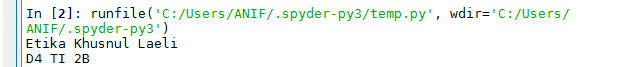
\includegraphics[width=4cm]{figures/1184065/RunFileVariable.PNG}
		\centering
		\caption{gambar diatas merupakan semacam pemberitahuan setelah kita menjalankan script pada variable explore apakah script yg dijalankan berhasil atau tidak }
	\end{figure}
	\begin{figure}[H]
		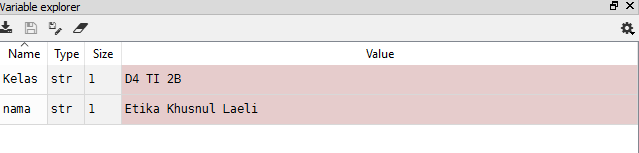
\includegraphics[width=4cm]{figures/1184065/ValueVariable.PNG}
		\centering
		\caption{gambar diatas merupakan hasil dari koding variable explorer yang terdapat nama,type,size dan value }
	\end{figure}
\subsection{Indentasi}
\begin{figure}[H]
		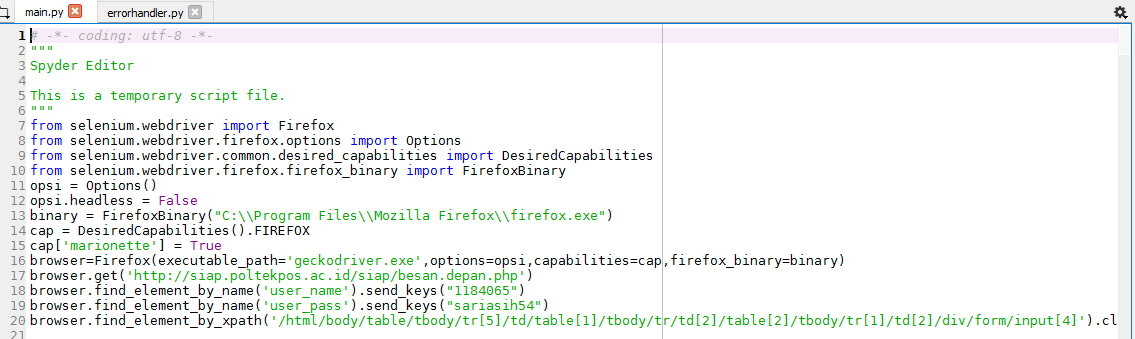
\includegraphics[width=4cm]{figures/1184065/KodingPenggunaOtomatis.PNG}
		\centering
		\caption{gambar diatas merupakan script contoh python pengguna selenium yang melibatkan inputan user.Jadi di dalam script tersebut kita sudah mengatur username serta password kita yang ada di SIAP.}
	\end{figure}
\subsubsection{Penjelasan Indentasi}
Indentasi dalam pemrogaman merupakan salah satu cara untuk merapihkan sintaks atau aturan dalam Bahasa pemrogaman yang hendak ditulis. Indentasi digunakan untuk acuan scope pemrogaman dan compiler seperti Bahasa pemrogaman python. Indentasi selalu ditandai atau berhubungan dengan kurung kurawal ‘{}’ untuk memulai atau mengakhiri suatu scope permasalahan. Indentasi seringkali menjadi salah satu kebiasaan dan ciri khas dari seorang programmer. Biasanya indentasi dipakai untuk sekedar memudahkan pembacaan kode program, namun dalam Python, indentasi berfungsi sebagai penanda blok kode program.
\subsubsection{Jenis-jenis error identasi yang didapat}
\begin{enumerate}
	\item penulisan script pada spyder tidak tepat pada posisi, misalnya penulisan yg kurang menjorok ke dalam atau terlalu menjorok
\end{enumerate}
\subsubsection{Cara membaca error}
\begin{enumerate}
	\item untuk membaca error kita dapat melihat di IPython Console, lihat error di bawah ini :
	\begin{figure}[H]
		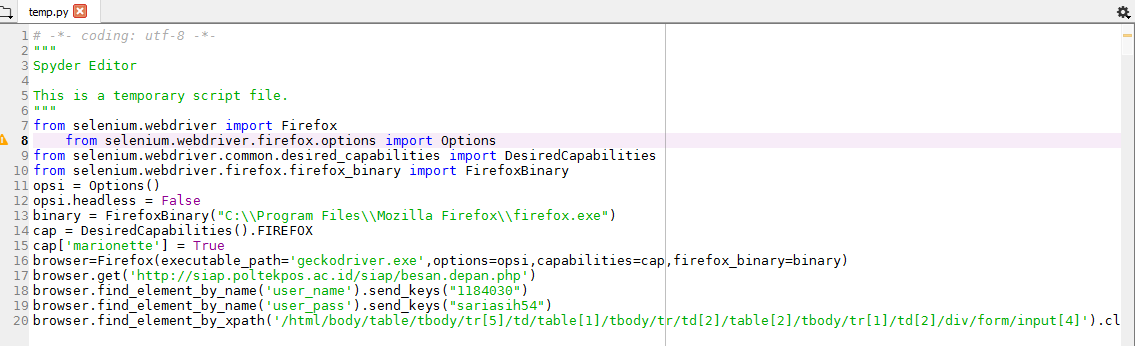
\includegraphics[width=4cm]{figures/1184065/ErrorSelenium1.PNG}
		\centering
		\caption{gambar diatas merupakan script contoh python pengguna selenium yang melibatkan inputan user dengan penulisan syntax pemrogaman salah karena terlalu menjorok ke dalam.}
	\end{figure}
	\begin{figure}[H]
		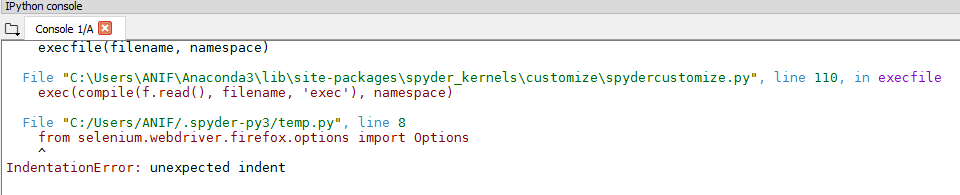
\includegraphics[width=4cm]{figures/1184065/PemberitahuanError1.PNG}
		\centering
		\caption{gambar diatas merupakan pemberitahuan dari syntax pemrogaman yang salah sehingga untuk membaca error kita dapat melihat pada bagian ini.}
		\end{figure}
\end{enumerate}
\subsubsection{Cara menangani error}
Untuk menangani error kita butuh melihat pada pemberitahuan errornya di compare lalu kita bisa memperbaikinya menjadi script yang benar hingga bisa masuk login secara otomatis pada web SIAP .
\begin{figure}[H]
		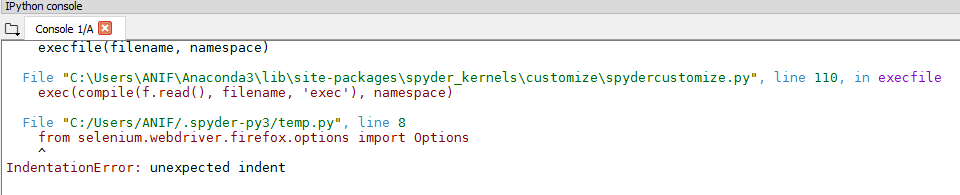
\includegraphics[width=4cm]{figures/1184065/PemberitahuanError1.PNG}
		\centering
		\caption{gambar diatas merupakan pemberitahuan dari syntax pemrogaman yang salah jadi untuk menanganinya kita melihat dari pemberitahuan ini.}
		\end{figure}
		\begin{figure}[H]
		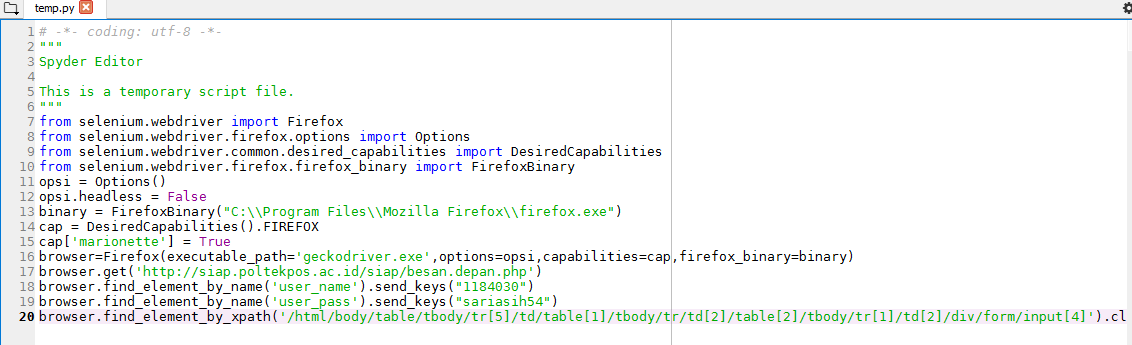
\includegraphics[width=4cm]{figures/1184065/MenanganiError1.PNG}
		\centering
		\caption{gambar diatas merupakan syntax yang sudah benar karena sudah di perbaiki yang bisa login otomatis ke dalam SIAP.}
		\end{figure}
		\begin{figure}[H]
		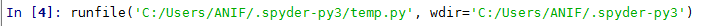
\includegraphics[width=4cm]{figures/1184065/PemberitahuanBenar1.PNG}
		\centering
		\caption{gambar diatas merupakan pemberitahuan dari syntax pemrogaman yang benar.}
		\end{figure}






	
